\documentclass[12pt]{article}
% Cross-references for handout numbers.
\usepackage{amsfonts}
%\usepackage{amsthm}
\usepackage{hyperref}
\usepackage{amssymb}
%\usepackage[capitalize]{cleveref}
\usepackage{xcolor}

%\input{handouts}

\newcounter{chapnum}

\newtheorem{definition}{Definition}[chapnum]
\newtheorem{remark}{Remark}[chapnum]
\newtheorem{theorem}{Theorem}[chapnum]
\newtheorem{lemma}[theorem]{Lemma}
\newtheorem{corollary}[theorem]{Corollary}
\newtheorem{proposition}[theorem]{Proposition}
\newtheorem{claim}[theorem]{Claim}
\newtheorem{observation}{Observation}[chapnum]

\renewcommand{\thesection}{\arabic{chapnum}.\arabic{section}}
\renewcommand{\thefigure}{\arabic{chapnum}.\arabic{figure}}


\newenvironment{proof}{\noindent{\bf Proof:} \hspace*{1em}}{
        \hspace*{\fill} $\triangle$ }
\newenvironment{proof_of}[1]{\noindent {\bf Proof of #1:}
        \hspace*{1em} }{\hspace*{\fill} $\triangle$ }
\newenvironment{proof_claim}{\begin{quotation} \noindent}{
        \hspace*{\fill} $\diamond$ \end{quotation}}
\newenvironment{solution}{\noindent{\bf Solution:} \hspace*{1em}}{
        \hspace*{\fill} $\triangle$ }


\newcommand{\R}{{\mathbb R}}
\newcommand{\Z}{{\mathbb Z}}
\newcommand{\Q}{{\mathbb Q}}
\newcommand{\C}{{\mathbb C}}
\newcommand{\N}{{\mathbb N}}
\newcommand{\lin}{\operatorname{lin}}
\newcommand{\aff}{\operatorname{aff}}
\newcommand{\cone}{\operatorname{cone}}
\newcommand{\conv}{\operatorname{conv}}
\newcommand{\vol}{\operatorname{vol}}
\newcommand{\poly}{\operatorname{poly}}




\newcommand{\CF}[1]{{\color{purple}[CF: #1]}}


\newlength{\toppush}
\setlength{\toppush}{2\headheight}
\addtolength{\toppush}{\headsep}

\newcommand{\htitle}[2]{\noindent\vspace*{-\toppush}\newline\parbox{6.5in}
{Massachusetts Institute of Technology \hfill 18.453: Combinatorial Optimization 
\newline
\textbf{Instructor:} Cole Franks \quad \textbf{Notes: }Michel Goemans and Zeb Brady \hfill#2\newline
\mbox{}\hrulefill\mbox{}}\vspace*{1ex}\mbox{}\newline
\begin{center}{\Large\bf #1}\end{center}}

\newcommand{\handout}[2]{\thispagestyle{empty}
 \markboth{ #1 \hfil #2}{ #1 \hfil #2}
 \pagestyle{myheadings}\htitle{#1}{#2}}


\setlength{\oddsidemargin}{0pt}
\setlength{\evensidemargin}{0pt}
\setlength{\textwidth}{6.5in}
\setlength{\topmargin}{0in}
\setlength{\textheight}{8.5in}


\newcounter{exercisenum}
\newcounter{exercisetot}
\setcounter{exercisetot}{0}



\newenvironment{exercises}{
	\begin{list}{{\bf Exercise \arabic{chapnum}-\arabic{exercisenum}. \hspace*{0.5em}}}
	{\setlength{\leftmargin}{0em}
	 \setlength{\rightmargin}{0em}
	 \setlength{\labelwidth}{0em}
	 \setlength{\labelsep}{0em}
	\usecounter{exercisenum}
      \setcounter{exercisenum}{\theexercisetot}}}{\setcounter{exercisetot}{\theexercisenum}\end{list}}


\newenvironment{pseudocode}{
    \begin{list}{}{
        \renewcommand{\makelabel}{$\triangleright$}
        \setlength{\topsep}{0pt}
        \setlength{\leftmargin}{32pt}
        \setlength{\labelwidth}{14pt}
        \setlength{\labelsep}{0mm}
        \setlength{\itemindent}{0mm}
        \setlength{\itemsep}{-3pt}
        \setlength{\itemsep}{0mm}
        \setlength{\parsep}{0pt}%
        \setlength{\listparindent}{0pt}
    }
}
{
    \end{list}
}

\usepackage{graphicx,../lp,amsmath}
\newcommand{\I}{\mathcal I}
\begin{document}


\handout{Solutions to some of the exercises}{Updated 2/5/2017}

% 2009
% ps1

%2013
% ps1: 1-2, 1-3, 1-4, 1-5 and 1-12. Grad: 1-8.
% ps2: 2-1, 2-2 and 2-3. 3-1, 3-2. Grad: 2-7.
% ps3: 3-9, 3-12 and 3-17. 4-2, 4-7 and 4-8. 

%2015
% ps1: 1-9

\begin{enumerate}
\item[1-2] % Cesar Cuenca
\begin{quote}
An {\it edge cover} of a graph $G=(V,E)$ is a subset of $R$ of $E$ such that
every vertex of $V$ is incident to at least one edge in $R$.  Let $G$
be a bipartite graph with no isolated vertex.  Show that the
cardinality of the minimum edge cover $R^*$ of $G$ is equal to $|V|$
minus the cardinality of the maximum matching $M^*$ of $G$.  Give an
efficient algorithm for finding the minimum edge cover of $G$. Is this
true also for non-bipartite graphs? 
\end{quote}

%%%%%%%%%%%
Let $\rho(G)$ be the size of a minimum edge cover
and $\nu(G)$ the size of the maximum matching. A maximum matching
covers $2 \nu(G)$ vertices. Because of the connectedness, the
remaining $n-2\nu(G)$ vertices can be covered by no more than $n
-2\nu(G)$ edges. These edges and the maximum matching thus form an
edge cover of size $n-\nu(G)$. On the other hand, a minimum edge
cover has to be a forest (an acyclic graph). (Indeed, if it has any
cycle then the removal of any edge of the cycle would still give an
edge cover, of smaller cardinality.)  The number of connected
components of this forest is precisely $n - \rho(G)$ because every
component of the forest is a tree, and a tree on $k$ vertices has $k-1$ edges,
and one can take one edge per component to get a matching. We therefore have
$\nu(G) \geq n-\rho(G)$.

The first part of the proof clearly yields an algorithm for finding a minimum edge cover
given an algorithm for finding a maximum cardinality matching.

Yes, the result remains true for non-bipartite graphs.
Observe the proof above carries over for non-bipartite graphs.

%
\item[1-3]
\begin{quote}
Show that in any graph $G=(V,E)$ (not necessarily bipartite), the size
of {\it any maximal} matching $M$ (i.e. a matching $M$ in which one
cannot add an edge while keeping it a matching) is at least half the
size of a {\it maximum} matching $M^*$. 
\end{quote}

Let $M^*$ be a maximum matching and $M$ a maximal
  one. For every edge $e \in M^*$, at least one of its endpoints must
  be covered by edges of $M$. Otherwise the edge $e$ can be added to
  $M$, which contradicts its maximality. It follows that the number of
  vertices covered by $M$ is at least the number of edges in $M^*$,
  thus $2|M| \geq |M^*|$.

\item[1-4]
\begin{quote}
Consider the problem of perfectly tiling a subset of a checkerboard
  (i.e. a collection of unit squares, see example below) with dominoes
  (a domino being 2 adjacent squares).
\begin{enumerate}
\item
Show that this problem can be formulated as the problem of deciding
whether a bipartite graph has a perfect matching. 
\item 
Can the following figure be tiled by dominoes? Give a tiling or
  a short proof that no tiling exists.

\begin{center}
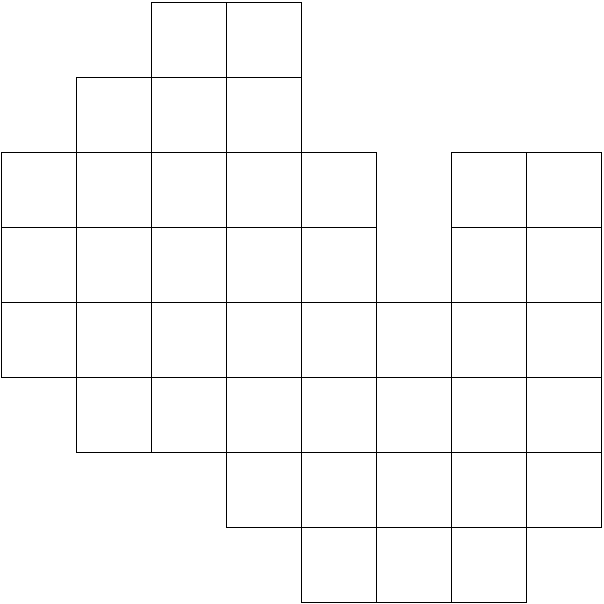
\includegraphics[height=2.5in]{../figures/domino}
\end{center}
\end{enumerate}
\end{quote}
%%%%%%%%%%%%%%%

\begin{enumerate}
\item Consider the bipartite graph $G$ with a vertex for each square
  and two squares are adjacent if they share an edge. This graph is
  bipartite since the squares can be colored black and white in a
  checkerboard pattern.

Any perfect tiling gives a perfect matching by simply selecting the
edges corresponding to the dominoes selected. And vice versa.
\item
\begin{figure}[ht]
\begin{center}
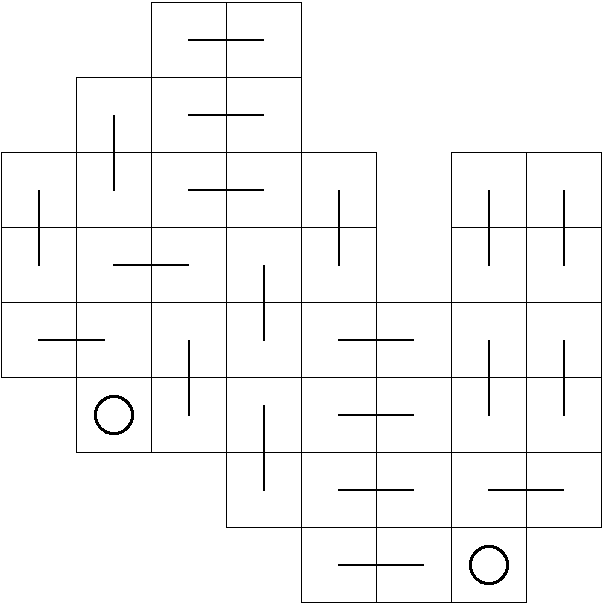
\includegraphics[height=2.3in]{../figures/domino2}
\end{center}
\caption{Maximum configuration of dominoes. \label{fig:domino2}}
\end{figure}

We claim that the configuration shown in Figure \ref{fig:domino2} is a
maximum one and so no perfect tiling exists. We will prove that the
matching $M$ corresponding to the configuration in Figure
\ref{fig:domino2} is maximum by showing that there is no augmenting
path as in the lecture. (Alternatively we could use Hall's theorem.)

Let $A$ be the set of black squares and $B$ the set of white squares.
Orient the edges of $G$ according to $M$, i.e. all the edges in $M$
are oriented from $B$ to $A$, and the edges not in $M$ are oriented
from $A$ to $B$ as in Figure \ref{fig:domino34}.

Let $v$ be the only exposed vertex of $A$ and $w$ be the only exposed
vertex of $B$, and consider $L$ to be the set of vertices reachable
from $v$ (the enclosed area in Figure \ref{fig:domino34}). Since $w$
is not in $L$ we obtain that no augmenting path exists.
\begin{figure}[ht]
\begin{minipage}[b]{0.5\linewidth} % A minipage that covers half the page
\begin{center}
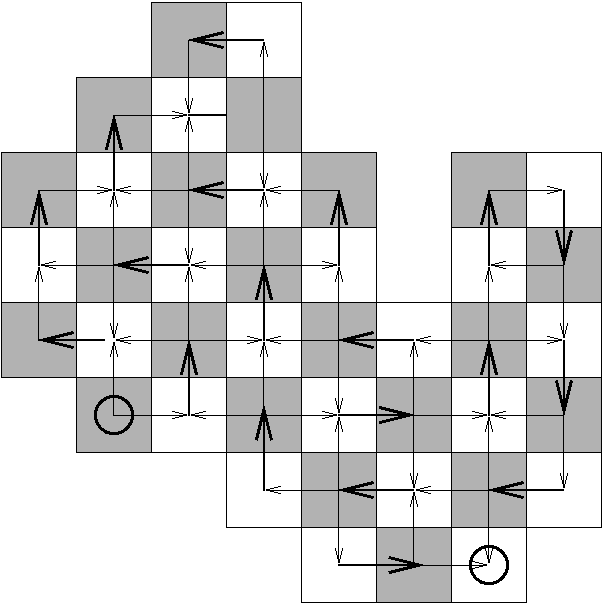
\includegraphics[height=2.3in]{../figures/domino3}
\end{center}
\caption{Oriented graph.}
\end{minipage}
\hspace{0.5cm} % To get a little bit of space between the figures
\begin{minipage}[b]{0.5\linewidth}
\begin{center}
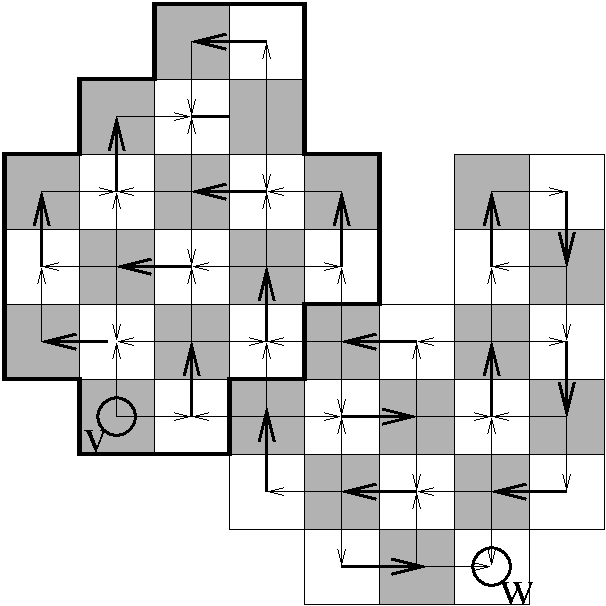
\includegraphics[height=2.3in]{../figures/domino4}
\end{center}
\caption{Set of reachable vertices from $v$.\label{fig:domino34}}
\end{minipage}
\end{figure}

We can also deduce the fact that no perfect matching exists from
Hall's theorem by observing that the 11 black vertices in $L$ (the
enclosed region on the right of Figure \ref{fig:domino34}) has only 10
(white) neighbors. 
\end{enumerate}
%%%%%%%%%%%%%%%%%%%%

\item[1-5]
\begin{quote}
Consider a $m\times n$ checkerboard where $m$ is even, and cells are alternatively colored black and white. Show that if we remove arbitrarily one black cell and one white cell, the resulting $mn-2$ cells can be covered by dominoes. 
\end{quote}

% see http://mathoverflow.net/questions/8846/proofs-without-words
% math gem 1; proof by Gomory

The $m\times n$ checkerboard when $m$ is even has a Hamiltonian cycle. After removing two cells of different colors, we get two even paths which can each be covered by a matching. 

\item[1-6] % Cesar Cuenca
\begin{quote}
% from Korte-Vygen's book
Consider a bipartite graph $G=(V,E)$ with bipartition $(A,B)$: $V=A
\cup B$. Assume that, for some vertex sets $A_1\subseteq A$ and $B_1
\subseteq B$, there exists a matching $M_A$ covering all vertices in
$A_1$ and a matching $M_B$ covering all vertices in $B_1$. Prove that
there always exists a matching covering all vertices in $A_1\cup
B_1$. 
\end{quote}
%%%%%%%%%%%%%%

% could also be proved using matching matroids, see later exercise
Let $G = (V, E) = (A\cup B, E)$, subsets $A_1 \subset A, B_1 \subset B$ and matchings
$M_A, M_B$ that cover $A_1$ and $B_1$, respectively.
We construct a matching $M$ that covers $A_1 \cup B_1$.
	
Clearly, the edge set $M = M_A \cup M_B$ covers $A_1 \cup B_1$, but it is not necessarily a matching.
We show how to delete edges from $M$ to make it into a matching.
We know $M_A \triangle M_B$ is a union of disjoint cycles and alternating paths.
The vertices with some incident edge from both $M_A\setminus M_B$ and from $M_B\setminus M_A$ are the only ones
where {\em $M$ fails to be a matching}.
We show how to delete some edges from $M_A \triangle M_B$, so $M$ is still a matching
and no vertices are uncovered. We do so in each component of $M_A \triangle M_B$.
	
\begin{itemize}
	
\item \textbf{Cycle:} Since $G$ is bipartite, the cycle has even length.
Therefore, we can delete every other edge and the desired properties hold.
		
\item \textbf{Path of odd number of edges:} We can delete every other edge
starting from the edge that is adjacent to the last edge of the path.
The desired properties hold.
Note that this is possible only because the path has odd number of edges.
		
\item \textbf{Path of even number of edges:} In this case, we can delete every other edge
but one endpoint will be covered and the other uncovered.
We need to prove that both endpoints cannot be in $A_1\cup B_1$.
Thus, we delete every other edge so the endpoint that is not in $A_1\cup B_1$ is uncovered.
		
We do so by contradiction: assume both endpoints are in $A_1\cup B_1$.
As the path has an even number of edges, and $G$ is bipartite, then both endpoints
must belong to the same bipartition set ($A$ or $B$).
W.l.o.g say they both belong to $A$, and thus also belong to $A_1$.
Note that each vertex in $A_1$ has exactly one incident edge from $M_A$;
thus the path we are analyzing (that is a connected component of $M_A \triangle M_B$)
must contain these two edges. However, this path is of even length,
and is alternating, so the end-edges cannot be from the same matching $M_A$ ($\Longrightarrow\Longleftarrow$).
This shows that our initial assumption is wrong, i.e., it must happen that
both endpoints do not belong to $A_1\cup B_1$, as desired.
\end{itemize}

\item[1-7] % from 2009
\begin{quote}
Consider a bipartite graph $G=(V,E)$ with bipartition $(A,B)$
($V=A\cup B$). Let ${\cal I}=\{X\subseteq A:$ there exists a matching
$M$ of $G$ such that all vertices of $X$ are matched$\}$. 

Show that 
\begin{enumerate}
\item
If $X\in {\cal I}$ and $Y\subseteq X$ then $Y\in {\cal I}$.
\item
If $X, Y\in {\cal I}$ and $|X|<|Y|$ then there exists $y\in Y\setminus
X$ such that $X\cup\{y\}\in {\cal I}$. 
\end{enumerate}
(Later in the class, we will discuss matroids, and properties (i) and
(ii) form the definition of independent sets of a matroid.)
\end{quote}
%%%%%%%%%%%%%%%

\begin{enumerate}
\item Let $Y \subset X \in {\cal I}$. Since $X$ is an
independent set, there exists a matching $M_X$ that covers $X$. This
matching also covers $Y$. Hence $Y$ is an independent set.
\item Let $X,Y \in {\cal I}$ with $|X| < |Y|$. It follows that
there exist matchings $M_X$ and $M_Y$ such that $M_X$ covers $X$ and
$M_Y$ covers $Y$. Consider the graph $G' = (V,M_X \Delta M_Y)$. The
set of edges of $G'$ is the union of paths and cycles.

If $M_X$ covers some element $y$ in $Y\setminus X$. Then $X+ y$ is an
independent set.

Otherwise, all the vertices in $Y\setminus X$ are of degree 1 in
$G'$. Since $|Y| > |X|$, we have $|Y\setminus X| > |X\setminus
Y|$. Therefore, by the previous observation, there are more degree 1
vertices in $Y\setminus X$ than in $X \setminus Y$. It follows that
there exists a path $P$ in the decomposition of $G'$ starting in a
vertex $y \in Y\setminus X$ and not ending in $X$. We conclude that
$M_X \Delta P$ is a matching of $G$ that covers $X \cup \{y\}$. Thus,
$X + y$ is an independent set.
\end{enumerate}

\item[1-8] % from 2007
\begin{quote}
% Slither game, ex p.144 in Cook et al.'s book
Consider the following 2-person game on a (not necessarily bipartite)
graph $G=(V,E)$. Players 1 and 2 alternate and each selects a (yet
unchosen) edge $e$ of the graph so that $e$ together with the
previously selected edges form a simple path. The first player unable
to select such an edge loses. Show that if $G$ has a {\it perfect}
matching then player 1 has a winning strategy. 
\end{quote}
%%%%%%%%%%%%%

Assume that there exists a perfect matching $M^*$
  in $G$. Then consider the following strategy for Player 1:
\begin{itemize}
\item In the first move, select any edge $e_o \in M^*$.
\item If Player 2 selects an edge $e = (v,w)$, where $w$ is a new
  endpoint of the path, then select the edge of $M^*$ that covers $w$.
\end{itemize}
	
It is easy to see that after every turn of Player 2, the path $P$
constructed so far is an even alternating path for $M^*$, and thus it
has only one vertex $w$ that has not been covered yet by edges of
$M^*\cap P$. Furthermore, this vertex must be an endpoint of the last
edge added by Player 2.  Since $M^*$ is a perfect matching, Player 1
can always add the edge of $M^*$ that covers $w$ to the path. The only
problem for this move could be that the new edge form a cycle, but
this is not possible since all the vertices in $V(P)\setminus \{w\}$
were already covered by edges of the matching.

Since Player 1 can always select an edge, he cannot lose, thus this is
a winning strategy.
%%%%%%%%%%
\item[1-9] % from 2007
\begin{quote}
Deduce Hall's theorem from K\"onig's theorem.
\end{quote}

%%%%%%%%%%%%

 It is easy to see that the condition is necessary.
  To see that it is sufficient, consider a (minimum) vertex cover $C$
  of size equal to the maximum matching, by means of K\"{o}nig's
  theorem and assume the condition given by Hall's theorem. For a
  contradiction, suppose that $|C|< |A|$. We have that $N(A
  \setminus C) \subseteq C \cap B$ (by definition of a vertex cover).
  Thus
\begin{align*}
  |N(A\setminus C)| \leq |C \cap B| =|C| - |C
  \cap A| < |A| - |C \cap A| = |A \setminus C|.
\end{align*}
This is a contradiction.

\item[1-10] % revised by Cesar Cuenca
\begin{quote}
Consider a bipartite graph $G=(V,E)$ with bipartition $(A,B)$. For
$X\subseteq A$, define $\operatorname{def}(X)=|X|-|N(X)|$ where $N(X)=\{b\in B:
\exists a\in X$ with $(a,b)\in E\}$. Let $$\operatorname{def}_{max}=
\max_{X\subseteq A} \operatorname{def}(X).$$ Since $\operatorname{def}(\emptyset)=0$, we have
$\operatorname{def}_{max}\geq 0$.  
\begin{enumerate}
\item
Generalize Hall's theorem by showing that the maximum size of a
matching in a bipartite graph $G$ equals $|A|-\operatorname{def}_{max}$. 
\item
For any 2 subsets $X, Y\subseteq A$, show that 
$$\operatorname{def}(X\cup Y) + \operatorname{def}(X\cap Y) \geq \operatorname{def}(X) + \operatorname{def}(Y).$$
\end{enumerate}
\end{quote}
%%%%%%%%%%%%%%%

\begin{enumerate}
\item
Clearly, the size of a maximum matching cannot be more than
$|A|-\operatorname{def}_{max}$ (since any matching has at
most $|A|-|X|$ edges incident to $A-X$ and at most $|N(X)|$ edges
incident to $X$).

Conversely, consider the minimum vertex cover $C$ and let
$X=A\setminus C$. Observe that $N(X)\subseteq C\cap B$, and thus
$$\operatorname{def}(X) =|X|-|N(X)|\geq |A\setminus C| - |C \cap B| =
|A| - |C \cap A|- |C\cap B|=|A|-|C|.$$  Therefore
$\operatorname{def}_{max}\geq |A|-|C|$ and the result follows from
K\"onig's theorem. 
\item
This is a simple counting argument. First of all, $$|X\cup Y|+|X\cap
Y|=|X|+|Y|.$$ Furthermore, $$|N(X\cup Y)| + |N(X\cap Y)| \leq |N(X)| +
|N(Y)|,$$ since every vertex $b$ in $B$ contributes at least as much
to the right-hand-side than to the left-hand-side. Indeed, if $b\in
N(X\cup Y)\setminus N(X\cap Y)$, it should be either in $N(X)$ or in
$N(Y)$, while if $b\in N(X \cap Y)$, it should be in both $N(X)$ and in $N(Y)$.
\end{enumerate}

\item[1-11] % from Chiheon?
\begin{quote}
Let $S=\{1,2, \cdots, n\}$. Let $A_k$ be the set of all subsets of $S$ of cardinality $k$ (thus $|A_k|={n \choose k}$). Let $k<\frac{n}{2}$. Consider the graph $G_k$ with bipartition $A_k$ and $A_{k+1}$, and with $E=\{(a,b) | a\in A_k, b\in A_{k+1}$ and $a\subset b\}$. 
\begin{enumerate}
\item
Prove that the maximum matching in $G_k$ has size $A_k$ (remember $k<n/2$). 
\item
Prove {\it Sperner's lemma}. The maximum number of subsets of $S$ such that no subset is contained into another is ${n \choose {\lfloor n/2 \rfloor}}$.  
\end{enumerate}
\end{quote}
%%%%%%%%%%%

\begin{enumerate}
\item Let $X$ be a subset of $A_k$. Note that any vertex in $A_k$ has degree $n-k$ in $G_k$. So, the number of edges between $X$ and $N(X)$ is $(n-k)|X|$. On the other hand, the number of edges adjacent to $N(X)$ is $(k+1)|N(X)|$ since any vertex in $A_{k+1}$ has degree $k+1$. Thus, $(n-k)|X| \leq (k+1)|N(X)|$. Since $k < \frac{n}{2}$, we have
$$
|X| \leq \frac{k+1}{n-k}|N(X)| \leq |N(X)|.
$$
By Hall's Theorem, there is a matching in $G_k$ covering $A_k$. 

\item For a collection $\mathcal{C}$ of subsets of $S$, we call it a {\it chain} if for any $x, y \in \mathcal{C}$ either $x \subset y$ or $y \subset x$. In other words, chain is a sequence of subsets $a_1 \subset a_2 \subset \dotsc \subset a_k$. On the other hand, we call a collection $\mathcal{F}$ of subsets of $S$ an {\it antichain}, if no subset is contained in another. Note that any chain and antichain can share at most one element. 

We claim that the collection of all subsets of $S$ can be partitioned into $\binom{n}{\lceil n/2 \rceil}$ chains. It implies that the size of antichain is at most $\binom{n}{\lceil n/2 \rceil}$, since antichain can have at most one element from each chain. 

Recall part (a). We know that $G_k$ has a matching covering $A_k$ if $k < \lceil \frac{n}{2} \rceil$. Similarly, if $k \geq \lceil \frac{n}{2} \rceil$ then $G_k$ has a matching covering $A_{k+1}$. Let $M$ be the union of those matchings in $G_k$ for $k=0,1,\dotsc,n-1$. Note that $M$ consists of disjoint paths, and for each path there are indices $k$ and $\ell$ such that the path is of the form $a_k a_{k+1} \dotsc a_\ell$ where $a_j \in A_j$ for $j=k, \dotsc, \ell$ and $a_j a_{j+1} \in M$. Moreover, each path contains exactly one element from $A_{\lceil \frac{n}{2} \rceil}$. Since each path is a chain, we have $\binom{n}{\lceil n/2 \rceil}$ disjoint chains covering all subsets of $S$. 


\end{enumerate}

%%%%%%%%%%%%%%%
\item[1-15]
\begin{quote}
Consider a bipartite graph $G=(V,E)$ in which every vertex has degree
$k$ (a so-called $k$-regular bipartite graph). Prove that such a graph
always has a perfect matching in two different ways:
\begin{enumerate}
\item
by using K\"onig's theorem,
\item
by using the linear programming formulation we have derived in this
section. 
\end{enumerate}
\end{quote}
%%%%%%%%%%%%%%%

Let $A$, $B$ be the bipartition of $V$.
\begin{enumerate}
  \item  Because of
  $k$-regularity, we have $|A| = |B|$. Let $n = |A|$.
  By K\"{o}nig's theorem, let $C$ be a minimum vertex cover of
  size equal to the maximum matching. Then, $N(A \setminus C)
  \subseteq B \cap C$, and because of $k$-regularity, $|A  \setminus C| \leq |B \cap C|$. Similarly, $|B
  \setminus C| \leq |A \cap C|$. Adding the inequalities we get $|V \setminus C|
  \leq |C|$, which implies  that $|C| \geq n$.

  \item Any integer solution of the LP formulation
    \lps
  &  &  & \mbox{Min} &  \sum_{i,j} c_{ij} x_{ij} \\
  & \lefteqn{\mbox{subject to:}} \\
  &        &   &  &   \sum_j x_{ij} =1 & i\in A \\
  &        &   &  &   \sum_i x_{ij} =1 & j\in B \\
  &        &   &  &  x_{ij}\geq 0 & i\in A, j\in B 
\elps  is a perfect  matching. Also, all the extreme points (if any) of the LP are integral (see
  lecture notes on bipartite matching).
  Thus, it is enough to prove that the LP is feasible (so it will have
  at least one extreme point), and this is indeed the case as $x_{ij}=
  1/k$ for all edges $(i,j)$ is a feasible solution.
\end{enumerate}
(One needs to add some assumption for the result to be true for non-bipartite graphs; indeed a cycle on 3 vertices does not have a perfect matching.)

%%%%%%%%%%%%%%
\item[1-17]
\begin{quote}
\item
Given a graph $G=(V,E)$, its edge coloring number is the smallest
number of colors needed to color the edges in $E$ so that any two
edges having a common endpoint have a different color. 
\begin{enumerate}
\item
Show that the edge coloring number of a {\it bipartite} graph $G$ is
always equal to its maximum degree $\Delta$ (i.e.~the maximum over all
vertices $v$ of the number of edges incident to $v$). (Use the
previous problem.) 
\item
Give an example of a non-bipartite graph for which the edge coloring
number is (strictly) greater than $\Delta$. 
\end{enumerate}
\end{quote}
%%%%%%%%%%%%%

\begin{enumerate}
\item
Clearly the edge coloring number is at least $\Delta$ since the
$\Delta$ edges incident to a vertex of maximum degree have to be
colored by different colors. To show the reverse inequality, first we
will transform  the graph $G$ into a $\Delta$-regular graph. For this
purpose, first add vertices if needed so that both sides of the
bipartition have the same number of vertices. Then add edges to the
graph (in any way) so that every vertex has now degree $\Delta$. In
the resulting graph $H$, we know by the previous exercise that there
exists a perfect matching. Deleting this perfect matching, we still
have a regular graph, now a $\Delta-1$-regular graph. We can therefore
again extract a perfect matching, delete it and proceed. In this
process, we have partitioned $H$ into $\Delta$ perfect matchings, and
thus the edges of $H$ can be colored with $\Delta$ colors. Since $G$
is a subgraph of $H$, restricting this coloring to the edges of $G$
gives a valid coloring with (at most, and thus exactly) $\Delta$ colors. 

\item
Consider a cycle on 3 vertices. 
\end{enumerate}

%%%%%%%%%%%%%%%%%%%
\item[2-2] % Cesar Cuenca
Let $G = (V,E)$, $S\subseteq V$ and a matching $M$ that covers $S$.
We construct a maximum matching $M^*$ that covers $S$ as follows.
Start with matching $M_0 = M$. In a general step, we have that if
$M_i$ is not maximum, then there exists an augmenting path $P_i$.
If we let $M_{i+1} = M_i \triangle P_i$, observe that the set
of covered vertices by $M_{i+1}$ includes the set of covered vertices
by $M_i$. We iterate this procedure until $M_n$ is a maximum matching, in which case we are done.

{\bf Observation:} We do not present an efficient algorithm
to find a desired maximum matching $M^{*}$ from $M$.
The statement of the problem does not ask for one.
%%%%%%%%%%%%%%%
\item[2-3] % revised by Cuenca
Let $U$ be a minimizer set and $M$ be a maximum
matching. Note that each edge in $M$ is either an edge of some
$G[K_i]$ or it is adjacent to some vertex in $U$. Also note that the
number of edges in $M$ adjacent to $U$ is at most $|U|$ and the number
of edges in $M$ from $G[K_i]$ is at most
$\left\lfloor\frac{|K_i|}{2}\right\rfloor$. It follows that:
\begin{align*}
|M| &= \left|\left[M \cap \{e \in E: e \text{ adjacent to some $v \in U$}\}\right]\right| +  \sum_{i=1}^k |M \cap E(G[K_k])|\\
&\leq |U| + \sum_{i=1}^k \left\lfloor\frac{|K_i|}{2}\right\rfloor = \frac{1}{2}(|V| + |U| - o(G\setminus U)) = |M|,
\end{align*}
where the last equality holds because $M$ is maximum and $U$ is
minimizer to the Tutte-Berge formula.

The previous formula implies that all the inequalities are equalities
(if some of them is strict, we would have a contradiction). In
particular we have that:
\begin{align*}
\left|\left[M \cap \{e \in E: e \text{ adjacent to some $v \in
U$}\}\right]\right| &= |U|, \\ \text{ and for every $i$, } |M \cap
E(G[K_k])| &= \left\lfloor\frac{|K_i|}{2}\right\rfloor .
\end{align*}

\begin{enumerate}
\item So $M$ has exactly $|U|$ edges adjacent to some vertex in
$U$, and for every~$i$, $M$ contains exacly
$\left\lfloor\frac{|K_i|}{2}\right\rfloor$ edges from $G[K_i]$. In
particular, $G[K_i]$ is perfectly matched for even components $K_i$
and near-perfect matched for odd components.

\item From the previous analysis, every vertex $u$ in $U$ is
matched to some vertex in $G \backslash U$. Since all the vertices of the even
components are already matched, $u$ must be matched to some vertex in
an odd component $K_i$ of $G\setminus U$.

\item Finally, since all the vertices in $U$ are matched to some vertex
outside $U$, and all the vertices in each even component are perfectly
matched, we obtain that the only unmatched vertices must be in odd
components of $G\setminus U$.
\end{enumerate}

%%%%%
\item[1-20]
\begin{quote}
%  Reingold Tarjan '81 SICOMP
  For the assignment problem, the greedy algorithm (which repeatedly
  finds the minimum cost edge disjoint from all the previously
  selected edges) can lead to a solution whose cost divided by the
  optimum cost can be arbitrarily large (even for graphs with 2
  vertices on each side of the bipartition).

Suppose now that the cost comes from a  metric, even just a line
metric. More precisely, suppose that the bipartition is $A \cup B$
with $|A|=|B|=n$ and the $i$th vertex of $A$ (resp. the $j$th vertex
of $B$) is associated with $a_i\in \R$ (resp. $b_j\in B$). Suppose
that the cost between these vertices is given by $c_{ij}=|a_i-b_j|$. 

Consider the greedy algorithm: select the closest pair of vertices,
one from $A$ and from $B$, match them together, delete them, and
repeat until all vertices are matched. For these line metric
instances, is the cost of the greedy solution always upper bounded by
a constant (independent of $n$) times the optimum cost of the
assignment? If so, prove it; if not, give a family of examples
(parametrized by $n$) such that the corresponding ratio becomes
arbitrarily large.
\end{quote}
%%%%%%%%%%

The greedy algorithm can provide solutions which are arbitrarily
  far away from the optimum. Reingold and Tarjan (SIAM J. on
  Computing, Vol. 10, 1981) show instances on a line for which the
  ratio between the greedy algorithm and the optimum cost matching is
  a factor more than $n^{0.58}$.


%%%%%%%%%%%%%%%%%
\iffalse
\item[2.6]
We will use the Tutte-Berge formula. Let $U \subseteq V$, and
let $W$ be any connected component of odd size of $G \setminus U$.
Because $G$ is 3-regular, there is an odd number of edges between
$W$ and $U$ (this follows by just counting the edges incident to a
vertex of $W$, and observing that the edges inside $W$ will be counted
twice). Moreover, those edges are a cutset. Thus, that cutset
has at least 3 edges. Because this is happening for every connected
component of odd size, the 3-regularity of $G$ implies that
$|U| \geq o(G \setminus U)$. In other words, by the
Tutte-Berge formula, $\max_M |M| = |V|/2$.

\fi
%%%%%%%%%%%%%%%%%%
\item[3-1]
We have: 

\begin{center}
$Ax=b, x\geq 0$ has no solution

iff

$Ax\leq b, -Ax \leq -b, -Ix\leq 0$ has no solution 

iff

$Cx\leq d$ has no solution where $C=\left(\begin{array}{c}A \\ -A
    \\ -I\end{array} \right)$ and $d=\left(\begin{array}{c}b \\ -b
    \\ 0\end{array} \right)$

iff

$\exists (p,q,r)\geq 0: A^Tp-A^Tq-Ir=0, b^Tp-b^Tq<0$

iff

$\exists (p,q)\geq 0: A^T(p-q)\geq 0, b^T(p-q)<0$

iff

$\exists y \geq 0: A^Ty\geq 0, b^Ty <0$.
\end{center}

%%%%%%%%%%%%%%
\item[3-2]   % Cesar Cuenca
Write the primal (P) in standard form
$$\max c^Tx$$
$$\textrm{s.t. }Ax\leq b$$
and its dual (D) as
$$\min b^Ty$$
$$\textrm{s.t. }A^Ty = c$$
$$y\geq 0$$
We can rewrite (D) by noting that $\min b^Ty = \max (-b^T)y$
and that $A^Ty = c$ is equivalent to $A^Ty \leq c$ and $-A^Ty \leq -c$.
$$\max(-b^T)y$$
$$\textrm{s.t. }
\begin{bmatrix}
A^T \\
-A^T\\
-I
\end{bmatrix}
y \leq
\begin{bmatrix}
c \\
-c\\
0
\end{bmatrix}
$$
Then the dual of (D) is (DD) below
$$\min \begin{bmatrix}
c^T & -c^T & 0
\end{bmatrix}y'$$
$$\textrm{s.t. }
\begin{bmatrix}
A & -A & -I
\end{bmatrix}
y' = -b$$
$$y'\geq 0$$
If in (P), $x\in\R^n, A\in\R^{m\times n}$, then $y\in\R^m \Longrightarrow y'\in\R^{2n+m}$.
Rewrite $y'$ as
$$y' = \begin{bmatrix}
x_{-} \\
x_{+}\\
z
\end{bmatrix},$$
where each $x_+, x_-$ has dimension $n$ and $z$ has dimension $m$; also let $x = x_+ - x_-$.
Thus, we can rewrite (DD) as
$$\min c^Tx_+ - c^Tx_-$$
$$\textrm{s.t. }Ax_+ - Ax_- - z = -b$$
$$x_+\geq 0$$
$$x_-\geq 0$$
$$z\geq 0,$$
or equivalently,
$$\max c^Tx$$
$$\textrm{s.t. }Ax + z = b$$
$$z\geq 0$$
Of course, this is equivalent to (P) since the last two constraints above
can be replaced by the single inequality $Ax \leq b$.
%%%%%%%%%%%%%
\iffalse
\item[3-8]
We know that every extreme point of a polytope is
  the unique solution for a system of equations obtained by selecting
  some of the inequalities defining the polytope and setting them as
  equalities. In particular, if $x^*$ is a vertex of $Q$, then there
  exists a subset $I$ of $\{1,\dots,m\}$, where $m$ is the number of
  rows of $A$, such that $x^*$ is the unique solution of the system
\begin{align*}
(Ax)_i &= b_i, \text{ for all $i \in I$}\\
Cx &= d.
\end{align*}
But this implies that $x^*$ is the unique solution for a system of
equations obtained by selecting some of the inequalities that define
$P$ and setting them as equalities. Since $x^* \in P$, it follows that
$x^*$ is an extreme point of $P$. Therefore, all the vertices of $Q$
are vertices of $P$.
\fi
%%%%%%%%%%%%%%%%%%%%%%
\item[3-9]
First consider the situation in which $M_1$ and $M_2$ are such that
$M_1\Delta M_2$ have more than one connected component. Consider one
of these connected components, say $S\subseteq V$, and partition $M_1$
and $M_2$ into $M_1=M_{1s}\cup M_{1t}$ and $M_2=M_{2s}\cup M_{2t}$
where $M_{1s}$ and $M_{2s}$ correspond to the edges within $S$. By
definition $M_{1s}\cup M_{2s}\neq \emptyset$. Now define two other
matchings by $M_3=M_{1s}\cup M_{2t}$ and $M_4=M_{2s}\cup
M_{1t}$. Observe that 
$$\chi(M_1) + \chi(M_2) = \chi(M_3)+\chi(M_4)$$
which implies that any face that contains $M_1$ and $M_2$ will also
contain $M_3$ and $M_4$, and thus cannot be an edge. 


Conversely, suppose that $M_1\Delta M_2$ has only one connected
component, and say that this component has $k_1$ edges from $M_1$ and
$k_2$ edges from $M_2$. We must have that $|k_1-k_2|\leq 1$. Now
consider the following cost function:
$$c_e=\left\{ \begin{array}{ll} 1 & e\in M_1\cap M_2 \\ -1 & e\notin
  (M_1\cup M_2) \\ k_2 & e\in M_1\setminus M_2 \\ k_1 & e\in
  M_2\setminus M_1.\end{array}\right.$$  Notice that $c(M_1)=c(M_2)=b$
where $b:=|M_1\cap M_2| + 2 k_1k_2$ and for any other matching $M$ we
have that $c(M)<b$. Thus the valid inequality $c^Tx \leq b$ induces a
face with only teh incidence vectors of $M_1$ and $M_2$ has
  vertices. Thus the line segment between $M_1$ and $M_2$ defines an
  edge. 

%%%%%%%%%%%%%%%%%%%%%
\iffalse
\item[3-11]
Consider the family of permutations
  $\{\sigma_1,\ldots,\sigma_n\}$ given by:
$$\sigma_i: \begin{cases}\sigma_i(1) = i,\\ \sigma_i(i)=1,\\ \sigma_i(j) = j, &j \notin \{1,i\}.\end{cases}$$
In other words, $\sigma_1$ is the identity permutation and $\sigma_i$
is the permutation that transpose $1$ and $i$. Let us prove that these
$n$ permutations are affinely independent. For that suppose that
$\lambda_1,\ldots, \lambda_n$ are real numbers such that:
$$\sum_{i=1}^n \lambda_i\sigma_i = 0, \quad \sum_{i=1}^n \lambda_i = 0.$$
Then for every $j\neq 1$:
\begin{align*}
 0 = \sum_{i=1}^n \lambda_i \sigma_i(j) &= \left(\sum_{i\neq j}\lambda_i \cdot j\right) + \lambda_j \cdot 1\\
 &= \left(\sum_{i=1}^n \lambda_i \cdot j \right) - \lambda_j \cdot j + \lambda_j \cdot 1\\
 &= \biggl(\underbrace{\sum_{i=1}^n \lambda_i}_{=0}\biggr) \cdot j  +\lambda_j \cdot (1-j).
\end{align*}
Hence, for every $j\neq 1$,\, $\lambda_j (1-j) = 0$, which implies
that $\lambda_j = 0$. Using that $\sum_{i=1}^n \lambda_i = 0$ we
deduce that $\lambda_1$ is also 0. Therefore, the family
$\{\sigma_1,\ldots,\sigma_n\}$ is a set of $n$ affinely independent
permutations.
\fi
%%%%%%%%%%%%%%%%%%%%%
\iffalse
\item[3-16]
From the description of the matching polytope, we know that the
maximum size of a matching in a bipartite graph $G$ is given by:
$$\nu(G)=\max\{1^Tx: Ax\leq 1, x\geq 0\},$$
where $1$ denotes a vector of all 1's and $A$ is the vertex-edge
incidence  matrix (i.e., it has a row
for each vertex and a column for each edge, and a 1 in this entry if
the edge is incident to the vertex). By LP duality we know that   
$$\nu(G)=\min\{1^Ty: A^T y\geq 1, y\geq 0\},$$
where $y$ has a component $y_v$ for each vertex $v$ of $V$.
Since $A$ is TUM (see Theorem 3.13) so is $A^T$. Thus this dual also
has an optimum solution $y$ that is integral. Furthermore, given the
constraints, it is useless to have $y_v>1$ and thus we can assume that
for each $v\in V$, we have that $y_v\in\{0,1\}$. We just need to
observe not that $A^Ty\geq 1$ is identical to saying that $C$ is a
vertex cover where $C=\{v\in V: y_v=1\}$, and that $1^Ty=|C|$. This
proves K\"onig's theorem.  
\fi
%%%%%%%%%%%%
\item[3-17]

Let $I_i = [t_i, u_i) \subseteq \R$ be the time interval of activity $i$.
\begin{enumerate}
\item
We could write the integer program:
\lps
 &  &  & \mbox{Max} &  \sum_i p_i x_i \\
 & \lefteqn{\mbox{subject to:}} \\
 &        &   &  &   x_i + x_j \leq 1 & \forall i,j: I_i \cap I_j \neq
\emptyset\\
 &        &   &  &  x_i \in \{0,1\} & \forall i.
\elps
And this would be correct for this subquestion. However, if we relax
the integrality constraints some of the extreme points may be
fractional (consider for example 3 identical intervals).

A better formulation as an integer program is: \lps
 &  &  & \mbox{Max} &  \sum_i p_i x_i \\
 & \lefteqn{\mbox{subject to:}} \\
 &        &   &  &   \sum_{j: t_i\in I_j} x_j  \leq 1 & \forall i \\
 &        &   &  &  x_i \in \{0,1\} & \forall i.
\elps
 This is a valid formulation of the problem as any feasible (integer)
 solution cannot have two intervals, say $I_k$ and $I_l$, that
 overlap; indeed the constraint for $i=k$ or for $i=l$ would be
 violated.

\item Sort the rows of $A$ according to the left endpoint $t_i$ that
defines them. This shows that $A$ has the ``consecutive ones
property'' along columns, that is, every column is simply a
(possible empty) group of zeros followed by a (possible empty) group
of ones followed by a (possibly empty) group of zeros. Indeed, for
the column that corresponds to $x_j$, we have a one in row $i$ if
$t_i\in I_j$, and this implies that the ones will be consecutive.

Now, we will show that any matrix with the consecutive ones property
is totally unimodular. Consider any square submatrix $T$ of $A$; it
also has the consecutive ones property. For every row of $T$ except
the last, subtract the next row. This operation doesn't change the
determinant, but leaves at most one 1 and one -1 in each column, while
making the others 0. If there is a column with exactly one nonzero
entry, then by expanding the determinant along that entry, we can
consider a smaller sized matrix $T$.  Otherwise, every column has
exactly one $1$ and one $-1$. If we pre-multiply such a matrix by the
all ones vector, we get the 0 vector.  That is, the matrix is singular
and the determinant is 0. This shows that in all cases the determinant
of $T$ is 0, 1 or -1.

\end{enumerate}

%%%%%%%%%%%


%%%%%%%%%%%%%
\iffalse
\item[3-18]
\begin{enumerate}
\item
Yes, the matrix is still TU; we use Theorem 3.14 to prove it. Indeed,
consider any subset $R$ of its rows. Either the last row of the same
matrix is not among those selected in $R$ and then the result follows
from Theorem 3.13. On the other hand, if the last row is in $R$, then
put it in $R_2$ and put all the other rows in $R_1$. The sum of the
rows in $R_1$ will be a vector with all components $0, 1,$ or $2$, and
once we substract the last row (with only 1's), we get a $\{0,+1,
-1\}$-vector, proving that the matrix is TUM. 
\item
This follows immediately from Theorem 3.12. 
\item
  Not true. Consider a complete bipartite graph with $|A|=|B|=2$ and
  let $E_1$ be one of the perfect matchings and $e_2$ the other (both
  $|E_1|$ and $|E_2|$ equal 2). Take $k=1$. The vector with
  $x_e=\frac{1}{2}$ for $e\in E_1\cup E_2$ satisfies all the given
  inequalities, but is not in the convex hull of matchings with at
  most $k$ edges from $E_1$.   
\end{enumerate}
\fi
%%%%%%%%%%%%%%
\iffalse
\item[4-1]
Suppose that a partition matroid is specified by $E=E_1\sqcup E_2
\cdots \sqcup E_l$ and

$\mathcal{I} = \{X \subseteq E: |X\cap E_i|\leq k_i ,  i=1,\cdots,l\}$,
where $k_i \leq |E_i|.$ For each $i=1,\ldots,l ,$ consider the sub
matroid  $M_i=(E_i,{\mathcal{I}}_i )$, where ${\mathcal{I}}_i=\{X\subseteq E_i
: |X|\leq k_i\}.$ Clearly if $A_i$ is a matrix that represents $M_i$
over $R,$ then the block diagonal matrix $A_1\bigoplus \cdots
\bigoplus A_l$ represents $M$ over $\mathbb{R}.$

It is easy to see that each $M_i$ is the uniform matroid
$U_{k_i,|E_i|}$.

Now, we only need to show that how we can represent the uniform
matroid $U_{k,n}$ over $\mathbb{R}.$ Take $v_1,\ldots,v_n \in
{\mathbb{R}}^{k}$, where $v_i=(1,i,i^{2},\ldots,i^{k-1}).$ Then any
subset of $\{v_1,\cdots,v_n\}$ of cardinality $k$ is independent due
to the Vandermonde determinant. On the other hand, any subset of
size greater than $k$ must be dependent since we are in
${\mathbb{R}}^{k}.$ So the matrix whose columns are $v_1,\ldots,v_n$
represents the uniform matroid $U_{k,n}.$

Therefore, the partition matroid $M$, represents by block diagonal
matrix, whose $i$-th block is isomorphic to the matrix representing
$U_{k_i,|E_i|}.$
\fi
%%%%%%%%%%%%%%%%%%
\item[4-2] % Cesar Cuenca
Let $G$ be any graph on the vertex set $V$. Let us define $E = V$
and $\I  = \{ S \subseteq E: S \text{ is covered by some matching } M\}$.
To prove $(E, \I)$ is a matroid, we need to verify two axioms.

($I_1$) If $Y \in \I$ and $X \subseteq Y$ then $X \in \I$.

If $M$ is a matching covering $Y$, since $X\subseteq Y$, then $M$ also covers $X$. By definition, $X\in\I$.
	
($I_2$) If $X \in \I$ and $Y \in \I$ and $|Y| > |X|$ then there exists $v \in Y\setminus X : X \cup \{v\} \in\I$

Let $M_X, M_Y$ be matchings covering $X$ and $Y$, respectively.
If there exists $v\in Y\setminus X$ such that $v$ is a vertex covered by $M_X$,
then clearly $X \cup \{v\} \in I$. Then let us assume such vertex $v$ does not exist.
This assumption allows us to say that a vertex covered by both $M_X$ and $M_Y$
is either in both $X$ and $Y$, in $X$ but not in $Y$, or in neither $X$ nor $Y$.
In other words, a vertex covered by $M_X$ and $M_Y$ cannot be in $Y \backslash X$.
We wish to find a matching $M_X'$ covering $X \cup \{v\}$, for some $v \in Y \backslash X$.\\

Consider the edges in $M_X \Delta M_Y$. We know they form cycles or simple paths.
Since $|Y| > |X|$, then some cycle or some path must have more vertices from $Y$ than from $X$.
In cycles, all vertices are covered by both $M_X$ and $M_Y$.
As determined above, this implies that they cannot be in $Y \backslash X$.
Similarly, we see that the inner vertices of a path cannot be in $Y \backslash X$.
Thus, some path $P$ has one of its endpoints $v$ belonging to $Y \backslash X$.
It is thus clear that $M_X' = M_X \triangle P$ is a matching covering $X \cup \{v\}$,
for $v \in Y \backslash X$, as desired.

%%%%%%%%%%%%%%%%%
%%%%%%
\iffalse
\item[4-5]
It is easy to see that the first axiom is
satisfied. For the second, consider the following bipartite graph: one
set of vertices is $A = \cup A_i$ and the other is $B = \{A_i: 1 \leq
i \leq n\}$. A pair of vertices $a \in A$ and $A_i \in B$ forms an
edge iff $a \in A_i$. There is a correspondence between partial
transversals of the family of sets and matchings of the graph: given a
matching, the corresponding partial transversal is given by all the
vertices in $A$ that have an edge of the matching incident to
them. Consider two transversals $X$, $Y$ such that $|X| <
|Y|$, with associated matchings with edges $M$ and $N$. Consider
the sets $Y \setminus X$ and $X \setminus Y$ and alternating paths in
$M \triangle N$ starting at vertices in $Y \setminus X$. Because of
the cardinality condition we have that $|Y \setminus X| > |X
\setminus Y|$, which implies that not all such alternating paths can
end at vertices in $X \setminus Y$, that is, there exists $a \in Y
\setminus X$ such that the alternating path in $M \triangle N$
starting from it ends at a vertex in $B$. Then $X \cup \{a\}$ is also
a partial transversal, as we can augment the matching $M$ by means of
the alternating path starting at $a$.
\fi

\item[4-7]
It is easy to see that $(E,\mathcal{I})$ satisfies the first axiom
$(I_1)$ that if $X\subseteq Y$ and $Y \in \mathcal{I}$, then $X \in
\mathcal{I}.$ For $(I_2),$ consider $X,Y \in \mathcal{I}$ and $|Y|>|X|$, in
order to show the second axiom $(I_2)$, we need to show that there
exists $e \in Y\setminus X$ such that $X \cup \{e\} \in \mathcal{I}.$ Let us call
a set $S \in \mathcal{F}$ maximal in $T \subseteq E$, $T\neq S$, if
$S\subset T$ and $S$ is not contained in any other element of
$\mathcal{F}$ that is properly contained in $T.$ Suppose that
$A_1,\ldots, A_n $ are the maximal sets in $E.$ Set $A^{*}=E
\backslash(A_1\cup \cdots A_n).$ Since $|Y|>|X|$, we must have
$|Y\cap A^{*}|>|X\cap A^{*}|,$ or $|Y\cap A_i|>|X\cap A_i|$ for some
$i.$ In case $|Y\cap A^{*}|>|X\cap A^{*}|$, there is an element $e
\in (Y\cap A^{*})\in (X\cap A^{*}),$ and $X \cup \{e\} \in \mathcal{I}.$
So we only need to study the case that $|Y\cap A_i|>|X\cap A_i|$ for
some $i.$ Without lost of generality we may assume $|Y\cap
A_1|>|X\cap A_1|.$

Let $B_1,\ldots,B_m$ be the maximal sets in $A_1$ and let
$B^{*}=A_1\backslash(B_1\cup \ldots B_m)$. Since $|Y\cap
A_1|>|X\cap A_1|$, we have $|Y\cap B^{*}|>|X\cap B^{*}|$ or $|Y\cap
B_i|>|X\cap B_i|$ for some $i$. Again if $|Y\cap B^{*}|>|X\cap
B^{*}|$, there is an element $e \in (Y\cap A^{*})\in (X\cap A^{*}),$
and $X \cup \{e\}\in \mathcal{I}.$ Otherwise we can repeat this process
for $B_i$ satisfying $|Y\cap B_i|>|X\cap B_i|$. Since the ground set
$E$ is finite, we can find the required $e$ in finite number of
steps, and we are done.
%%%%%%%%%%%%%%%%%%%%%
\item[4-8] %revised by Cesar Cuenca
Let $(j_1, j_2, ..., j_k)$ be a sequence of jobs ordered in increasing order on their deadlines, i.e., $d_{j_1}\leq d_{j_2}\leq \ldots\leq d_{j_k}$. If they could not be completed in time, there must exist some $i$ for which $d_{j_i} < i$ (because $j_1$ will finish at time 1, $j_2$ will finish at time 2, etc.) However, this would imply that $d_{j_1}, d_{j_2}, ... d_{j_i} < i$.
	In other words, there are $i$ jobs with deadline less than $i$; therefore at least $i$ jobs need to be completed by the time $i-1$. This implies that the sequence of jobs is infeasible. Thus the contrapositive of what we just proved is that if a sequence of jobs can be completed in some order, then they can be completed in order of their deadlines.

Now we prove $M$ is a matroid by checking the two axioms.
		
{\bf I1} If $Y \in \I$ and $X \subset Y$, then $X \in I$.
	
This is obvious: if a set of jobs can be completed in time, then a subset of the jobs can also be completed in time.
	
{\bf I2} If $X \in I, Y \in I$ and $|Y| > |X|$ then $\exists e \in Y\setminus X : X \cup \{e\} \in I$.
	
Suppose both sets of jobs are ordered by deadline. Let $y  = |Y|, x = |X|$ and $e$ be one of the jobs with latest deadline in $Y \setminus X$. Suppose $e$ is in position $y-k$ of $Y$. Let $K = \{ j_{i_1}, j_{i_2}, ..., j_{i_k}\}$ be the set of jobs ordered by deadline ($d_{i_1} \leq d_{i_2} \leq ... \leq d_{i_k}$) that appear after $e$ in $Y$.
	
Since $e$ is in position $y-k$ in $Y$, we have $d_e \geq y-k$. Also $d_{i_t} \geq y - k + t$ because $j_{i_t}$ is in position $y - k + t$. In order to prove $X+e\in\I$, we need to prove there is no $q$ for which the job in position $q$ in $X$ has deadline $q$ for $q \geq d_e$ (This is the only way for $X+e$ to be infeasible.) For the sake of contradiction, assume such $q$ exists and job is $x_q$. Suppose there are $n$ elements from $K$ to the right of $x_q$. 
	
If $n = k$, then $x_q$ has at least $k$ elements to its right. This means that it is in position at most $x-k$. However, $x-k < y-k \leq q$. This is a contradiciton since $x_q$ is in position $q$ in $X$.
	
If $n < k$, then $x_q$ is to the right of $j_{i_{k-n}}$, which has deadline $d_{i_{k-n}} \geq y - k + (k-n) = y-n$. Therefore the deadline of $x_q$, which is $q$, satisfies $q \geq y-n > x-n$. However, since there are at least $n$ elements to the right of the $q$ element of $X$, we have $q \leq x-n$. Again a contradiction.
	
The contradiction proves that $X + e\in\I$, as desired.
	
Finally, to find an optimal scheduling, consider the value of each job $j_i$ being its reward $c_i$.
The greedy algorithm in matroid $M$ then finds the optimal configuration.
%%%%%%%%%%%%%%%%%%%%%
\iffalse
\item[4-8] %older version subsumed by solution above
Let $(j_1, \dotsc, j_k )$ be a sequence of jobs that can be
completed on time in that order. That is, $d_{j_i} \geq i$ for all
$i$. Suppose that two adjacent jobs from the sequence are not in the
order of their deadlines, that is, $d_{j_i} > d_{j_{i+1}}$. Then,
they can be swapped without breaking feasibility: $d_{j_i} >
d_{j_{i+1}} \geq i+1$. Thus, we can sort the list according to
increasing deadlines, while staying feasible.

We will now prove that $M$ is a matroid. Clearly $X \subseteq Y \in
\mathcal{I} \implies X \in \mathcal{I}$. For $(I_2)$, let $X,Y \in \mathcal{I}$,
$|Y| > |X|$. Let $e \in Y \setminus X$ be the job having the
latest deadline. Then $d_e \geq |Y| > |X|$ and it can be
added to $X$ without breaking feasibility.

To find an optimal ordering of the jobs, we can assume $c_j > 0$ for
all $j$ and use the greedy algorithm.
\fi
%%%%%%%%%%%%%%%%%%
\iffalse
\item[4-10]
For any $X \subseteq E$, let ${\mathcal{F}}_X= \{A\cap X: A\in
\mathcal{F}\}$; if we assume wlog that $E\in \mathcal{ F}$ then $X$
  is also in $\mathcal{F}_X$. We can see ${\mathcal{F}}_X$ is also a laminar
family of sets. Call a set $S \in {\mathcal{F}}_X$, $X$-maximal in
$T\subseteq E $ if $S\subset T$ and $S$ is not contained in any
other set in ${\mathcal{F}}_X$ that is properly contained in $T$.
For each $T \in {\mathcal{F}}_X$, let $T_1,\ldots,T_{n_{T}}$ be
$X$-maximal sets in $T$ and let $T^{*}=T\backslash(T_1\cup\ldots
\cup T_{n_T}).$ Then the rank of $T$ satisfies

\begin{equation}
r(T)=\min\{r(T_1)+\cdots+r(T_{n_{T}})+|T^{*}|, \min_{A\in \mathcal{F}: T\subseteq A} k(A) \},
\end{equation}
and this recursive formula also applies to $X$. 
\fi

%%%%%%%%%%%%%%%%%%%%%
\iffalse
\item[4-12]
First, let us prove that the conditions are sufficient.

Consider two independent set $I_1$ and $I_2$ such that (i) holds. Let $f$ be the only element in $I_2\setminus I_1$, and consider the weight function $c: E \to \R$ given by:
$$c(e)= \begin{cases}
1, &\text{if $e \in I_1$,}\\
0, &\text{if $e=f$,}\\
-1, &\text{if $e \notin I_2$.}
\end{cases}$$
For this cost, the only maximum weight independent sets are exactly $I_1$ and $I_2$. Therefore $I_1$ and $I_2$ are adjacent. The case where (ii) holds is analogous.

Now, assume that $I_1$ and $I_2$ satisfy (iii). For this case let $f$ be the only element in $I_2\setminus I_1$ and $g$ be the only element in $I_1\setminus I_2$. Consider the weight function $c: E \to \R$ given by:
$$c(e)= \begin{cases}
2, &\text{if $e \in I_1 \cap I_2$,}\\
1, &\text{if $e=f$, or $e=g$}\\
-1, &\text{if $e \notin I_1\cup I_2$.}
\end{cases}$$
For this cost, the only maximum weight independent sets are exactly $I_1$ and $I_2$, and so they are adjacent in the matroid polytope.

Now let us prove that the conditions are necessary.
  
  Assume that $I_1$ and $I_2$ are a pair of adjacent independent sets and let $c: E \to \R$ be a cost function  that is maximized only by $I_1$ and $I_2$. In particular note that $c(e) \geq 0$ for every element in $I_1 \cup I_2$. Assume w.l.o.g. that $|I_1| \leq |I_2|$.

\textbf{Case 1:}$|I_2| > |I_1|$. By the exchange axiom $(I3)$, there exists an element $f \in I_2\setminus I_1$ such that $I_1 + f$ is an independent set and, by a previous observation, it has weight greater or equal than the weight of $I_1$. Since $I_1$ is optimum it follows that so is $I_1 + f$. Since $I_2$ and $I_1$ are the only optimums, it follows that $I_2 = I_1 + f$. Therefore, (i) holds.

\textbf{Case 2:} $|I_2| = |I_1|$. Let $f$ be the element in $I_1\Delta I_2 = I_1\setminus I_2 \cup I_2 \setminus I_1$ with minimum cost. Assume w.l.o.g. that $f \in I_1$. Clearly, $I_1 - f$ is an independent set and $|I_1 - f| < |I_2|$. It follows that there exists an element $g \in I_2 \setminus I_1$ such that $I_1 - f + g$ is an independent set. By  choice of $f$, $c(I_1 -f + g) = c(I_1) - c(f) + c(g) \geq c(I_1)$. But then $I_1 - f + g$ is also a maximum weight independent set. Since $I_2$ and $I_1$ were the only optimums, it follows that $I_2 = I_1 - f + g$, which implies that $|I_2 \setminus I_1| = |I_2 \setminus I_2| = 1$. 

To conclude that (iii) holds, we only need to show that $I_1 \cup I_2 \not\in \mathcal{I}$. But this is easy to see since, in other case, using that $c(e) \geq 0$ for every $e \in I_1 \cup I_2$, we would have that $c(I_1 \cup I_2) \geq c(I_1)$. This implies that $I_1 \cup I_2$ is another optimum (different from $I_1$ and $I_2$), which contradicts the adjacency condition of $I_1$ and $I_2$.
\fi

%%%%%%%%%%%%%%%%%%%%%%%
% from Cesar Cuenca
\item[PS4-1/13] Problem 1 from Problem Set 4 from 2013. 

The set of sources is $So = \{f, i\}$, the set of sinks is $Si = \{e, h\}$.
In the exchange graph, one needs to find a path of minimum distance from
$So$ to $Si$, for example, $P = f \rightarrow a \rightarrow h$.
From this path, the larger independent set obtained is $S \triangle P = \{b, c, d, f, h\}$.

%%%%%%%%%%%%%%%%%%%%%%%%%%%%%%%%%
% from Cesar Cuenca
\item[5-1]
Our goal is to prove Konig's theorem using the matroid intersection theorem.
Recall that Konig's theorem states that if $G = (A\cup B, E)$ is a bipartite graph,
then the size of its maximum matching equals the size of its minimum vertex cover.

Consider $M_A = (E, \I_A)$ to be the matroid on the set of edges with
$\I_A = \{I \subset E : |\delta(v) \cap I| \leq 1 \textrm{ for all } v\in A\}$.
Define $M_B = (E, \I_B)$ similarly with $B$ replacing $A$.
The correspondence between an independent set in both matroids, i.e., an element
$I \in \I_A\cap\I_B$, and a matching of $M$.
Thus $\max_{S \in I_1\cap I_2} |S|$ is the size of the maximum matching in $G$.
We use the matroid intersection theorem with the matroids $M_A, M_B$, thus obtaining

$$
\max_{S \in \I_A\cap \I_B} |S| = 
\min_{U\subset E} [r_A(U) + r_B(E\setminus U)]
$$

We only need to show that the right hand side of the above expression equals the size of the minimum vertex cover in $G$.
Observe that both $M_A, M_B$ are partition matroids, for which we know the rank function.
In this case, for any $U\subset E$, $r_A(U)$ is the number of vertices of $A$ adjacent to some edge of $U$.
Let $A(U) \subset A$ be this set of vertices adjacent to some $e\in U$.
Likewise, $r_B(E\setminus U)$ is the number of vertices of $B$ NOT adjacent to any edge of $U$
and let $B(U) \subset B$ to this set of vertices. It is clear that $A(U) \cup B(U)$
is a vertex cover of $G$ of size $r_A(U) + r_B(E\setminus U)$.
This shows that the right hand side of the equation is at least the size of the minimum vertex cover.
Thus, we have proven that the size of the maximum matching is at least the size of the minimum vertex cover.
The other inequality is obvious (and indeed holds for any non-necessarily bipartite graph), so Konig's theorem follows.

%%%%%%%%%%%%%%%%%
% from Cesar Cuenca
\item[PS5-1-/13] Problem 1 from Problem Set 5 from 2013. 

Notice that one can begin by checking whether $w_i > w_n + g'$, where $g' = \sum_{i=1}^{n-1}{g_{ni}}$, for some $i < n$.
Obviously if this was the case, team $n$ could not win. Therefore, let us assume $w_i \leq w_n + \sum_{i=1}^{n-1}{g_{ni}}$ for all $i<n$.
Moreover, if there was an outcome where team $n$ won, then it could only get better if it won all of its games,
so let us assume that all $g_{ni}$ games to be played between teams $n$ and $i$ are won by team $n$.
If we let $x_{ij}$ to be the number of games between $i$ and $j$ won by $i$, then team $n$
has a chance of winning iff there are positive integers $x_{ij}$ with $x_{ij} + x_{ji} = g_{ij} = g_{ji}$,
$i\neq j$, and $w_i + \sum_{j=1}^{n-1}{x_{ij}} \leq w_n + g'$ for all $i<n$.

Consider the graph $G$ on $V = \{s, t\} \cup \{v(i, j)\}_{1 \leq i < j \leq n-1} \cup \{w(i)\}_{1 \leq i \leq n-1}$
with edges classified in these categories (all lower capacities are $l(e) = 0$).

\begin{itemize}
	\item All edges $e$ from $s$ to $v(i, j)$ with $u(e) = g_{ij}$.
	\item All edges $e_1, e_2$ from $v(i, j)$ to $w(i)$ and to $w(j)$ with $u(e_1) = u(e_2) = \infty$.
	\item All edges $e$ from $w(i)$ to $t$ with $u(e) = w_n + g' - w_i$.
\end{itemize}

We claim that team $n$ can win iff the maximum flow from $s$ to $t$ is $\sum_{i<j}{g_{ij}}$.
Indeed a maximum flow with that value exists iff there exists an integer flow $x: E \rightarrow \Z$
with that flow value exists (since all capacities are integers).
If we let $y_{ij} = x(v(i, j), w(i))$, such integer flow satisfies $y_{ij} \geq 0$, $g_{ij} = y_{ij} + y_{ji}$
and $\sum_{j=1}^{n-1}{x_{ij}} \leq w_n + g' - w_i$. As asserted above, this is equivalent to team $n$ having some chance.\\

%%%%%%%%%%%%%%
% Cesar Cuenca
\item[PS5-3/13] Problem 3 from Problem Set 5 from 2013. 

Let $G$ be an undirected graph with minimum degree $\delta(G) \geq k$.
We can consider $G$ as a digraph by replacing an edge $\{u, v\}$ by two arcs $(u, v), (v, u)$ with all $l(e) = 0$ and $u(e) = 1$.
We know that we can find $k$ edge-disjoint paths between vertices $s \neq t$ from an integral flow from $s$ to $t$ of value at least $k$.
Thus it will be enough to find two vertices $s, t$ and a flow with value at least $k$ between them.

Consider the following algorithm. Choose any vertex $v_1 \in V$ and let $S = \{v_1\}$.
Iteratively, find $v_i = \arg \max_{v\in V \setminus S}{c(S, \{v\})}$ and let $S = S\cup\{v_i\}$.
We get an ordering of the vertices $v_1, v_2, \ldots, v_n$.
As shown in the lecture notes, $\{v_n\}$ induces a minimum $(v_{n-1}, v_n)$-cut; the value
of such minimum cut equals to the outdegree of $v_n$, which is at least $k$ by assumption.
From duality, the maximum flow value between $v_{n-1}$ and $v_n$ is at least $k$, as desired.

%%%%%%%%%%%%%%%%%

%%%%%%%%%%%%%%%%%
\end{enumerate}
\end{document}
